\section{Pojačano učenje}
Najistaknutije osobine pojačanog učenja su pokušaj i neuspjeh, te odgođena nagrada koju algoritam doživljava u okruženju. Algoritam bi trebao, do neke razine, imati osjećaj i informacije o okolini, te cilj ili ciljeve prema kojima teži, a odnose se na određeno stanje u okolini.

\subsection{Umjetna inteligencija}
Umjetna inteligencija je jako široko područje računalne znanosti. Bavi se proučavanjem i izradom algoritama koji nemaju eksplicitne naredbe kako se ponašati u nekom trenutku i/ili okolini, nego kroz određene procese sami uspiju donijeti zaključke i odluke. Umjetna inteligencija se dijeli u puno pod grana, koje se u prošlosti nisu smatrali toliko srdonim koliko danas. U današnje doba se iskazao potencijal umjetne inteligencije i sve više se ulaže u njezino istraživanje i razvoj. 

Umjetna inteligencija se dijeli na više grana kao što su:
\begin{itemize}
	\item Rasuđivanje i rješavanje problema: Gdje se pokušava implementirati razbijanje problema u logičke korake do rješenja te postepenim izvršavanjem tih koraka riješiti zadani problem. Ovakvi algoritmi se nisu iskazali korisnima u velikim problemima zbog kombinatorijske eksplozije, znači rastom problema algoritam eksponencijalno usporava.
	
	\item Reprezentacija znanja: Ovo je glavno područje u istraživanju klasične umjetne inteligencije. Skupljaju se znanja od nekog područja i pohranjuju se u neku bazu u kojoj se istaknu pojmovi i veze između njih. Neke od stvari koje se nalaze u takvoj bazi su: predmeti, svojstva, vrste i odnosi između predmeta, situacija, događaja, stanja i vremena, uzroci i posljedice, znanje o znanju i još puno onih manje istraženih područja.
	
	\item Planiranje: Odnosi se na predviđanje nekih budućih događaja te donošenje određenih odluka koje utječu na ishod.
	
	\item Učenje: Predstavlja algoritme koji ispočetka jako loše rješavaju zadatak, međutim skupljanjem iskustva vremenom su sve bolji.
	
	\item Obrada prirodnog jezika: Omogućuje strojevima razumijevanje ljudskih jezika.
	
	\item Percepcija: Sposobnost pomoću određenih senzora primiti informacije o stvarnoj okolini te uspješno interpretirati te informacije u svoje zadaće.
	
	\item Kretanje i rukovanje: Upravljanje mehaničkih udova kako bi se riješio neki zadatak u stvarnoj okolini. Smatra se posebno kompleksnim, te obuhvaća paradoksni pojam (Moravec's paradox) u kojemu je teže implementirati radnju koju mlado dijete može izvoditi bez ikakvih poteškoća kao npr: primiti neki predmet u ruke i odložiti ga na određeni položaj od radnje kojoj je odraslome čovjeku teško kao npr: jako dobro odigrati partiju šaha. Izlazi iz činjenice da za razliku od šaha percepcija, kretanje i rukovanje su prirodnom selekcijom kroz milijune godina usađeni u čovjeka.
	
	\item Socijalna inteligencija: Uključuje poznavanje i prepoznavanje emocije i ljudskih međudjelovanja. Nekim algoritmima bi bilo vrlo korisno da uz pojmove teorije uključuje spoznaju ljudskih emotivnih stanja i motive za donijeti bolje odluke.
	
	\item Opća inteligencija: U prošlosti se pokušalo dizajnirati opće inteligentnog agenta koji pokriva široku ljudsku spoznaju. No odustalo se od toga, zbog preogromne količine informacija koje su kombinirane iz raznih područja. Danas se razvija 'usku' umjetnu inteligenciju koja je usredotočena u jedno područje i smatra se da opća umjetna inteligencija bi trebala ujediniti hrpu tih usredotočenih područja.
\end{itemize}

\subsection{Strojno učenje}
U ovome završnom radu se razradilo područje iz učenja. Pa tako se i ovo područje grana na više potpodručja. Među najpoznatijima su učenje s nazorom (eng. \textit{supervised learning}) u kojemu algoritam dobije skup podataka iz kojih treba donijet neke zaključke, te skup rješenja, odnosno definirane zaključke koje bi trebao donijeti. Tako da kroz neko vrijeme koje je dodijeljeno za učenje, primi podatak, donese odluku i ovisno 
o tome koji je unaprijed definirani zaključak kojeg je trebao donijeti se prilagodi da u buduće donosi što ispravnije odluke. Druga grana se zove učenje bez nazora (eng. \textit{unsupervised learning}), gdje algoritam prima neki skup podataka i vremenom uspije pronaći razlike i sličnosti u podacima. Nema informacije o tome što podatak predstavlja ali zna podatke svrstati u svoje definirane kategorije. Izrađeni agent iz ovog projekta spada pod skupinom pojačanog učenja (eng. \textit{reinforcement learning}). U ovoj grani algoritam djeluje u nekom okruženju pomoću određenih akcija, te u početku nema informacije o tome kako akcije utječu na okruženje. Te vremenom mora sam otkriti koje akcije u kojem trenutku donose najveću nagradu.


\subsection{Povijest pojačanog učenja}
Što se tiče povijesti pojačanog učenja vrijedi spomenuti dvije glavne grane koje su tada postojale kao samostalne dok se danas isprepliću. Jedna od njih je nastala kao dio psihologije životinjskog učenja te se fokusirala na učenje metodom pokušaja i pogreške. Druga pak koristi vrijednosne funkcije i dinamičko programiranje te se bavi problemom optimalnog upravljanja i njegovog rješenja. Prva grana pojačanog učenja je zapravo i dovela do otkrića pojačanog učenja početkom 1980-tih godina te se može reći kako kao takva proizlazi iz nekih najranijih djela umjetne inteligencije, iako se sama ideja takvog načina učenja, metode pokušaja i pogreške, proteže unazad čak do 1850-tih godina. Edward Thorndike je bio prvi koji je uspio objasniti bit učenja metodom pokušaja i pogreške te ju je nazvao "Zakon učinka" (eng. \textit{Law of effect}): "Od nekoliko odgovora danih na istu situaciju, oni koji su povezani ili pomno prate životinjsku volju, pod jednakim uvjetima, čvršće će biti povezani sa situacijom, tako da će, kad se ponovi, biti vjerojatnije da će se i oni ponoviti; oni koji su povezani ili pomno prate nelagodu životinje, pod jednakim uvjetima, imat će oslabljene veze s tom situacijom, pa će, kada se ponovi, biti manje vjerojatno da će se i ona ponoviti"~\cite{reinforcement_learning}.

Alan Turing je opisao sistem „zadovoljstvo – patnja” koji je funkcionirao u skladu sa Zakonom učinka. To je ujedno bila i jedna od najranijih ideja kako implementirati metodu pokušaja i učenja s umjetnom inteligencijom. Kod druge metode, pojam "optimalna kontrola" počeo se upotrebljavati za opisivanje problema dizajniranja regulatora koji minimalizira ili maksimizira mjeru ponašanja dinamičkog sustava tijekom vremena. Dinamičko programiranje smatra se jedinim izvedivim načinom rješavanja općenito stohastičkih problema optimalnog upravljanja. I dalje je učinkovitiji i više se primjenjuje od ijedne druge opće metode iako njezini računski zahtjevi eksponencijalno rastu s brojem varijabli stanja. Puno vremena je trebalo da bi se prepoznavale veze između optimalne kontrole i dinamičkog programiranja i učenja. Postupak djelovanja na pojačano učenje pomoću MDP (Markov Decision Processes) formalizma s kojim je radio Chris Watkins 1989. godine je zapravo vrijeme kada se dogodila potpuna integracija metoda dinamičkog programiranja s učenjem za vrijeme dobivanja novih podataka. Ove dvije glavne grane pojačanog učenja su se u kasnim 1980-tim godinama međusobno povezale s trećom, manje izraženom granom, koja se bavi metodom vremenske razlike.

\subsection{Elementi pojačanog učenja}
Osnovni građevni blokovi na kojem se temelje metode pojačanog učenja su:
\begin{itemize}
	\item Politika: Opisuje ponašanje u određenom trenutku. Određuje koje radnje poduzeti ovisno o stanju okruženja, iskazuje se kao funkcija vjerojatnosti koja opisuje vjerojatnost sljedeće određene radnje.
	
	\item Signal nagrade: Govori algoritmu koliko je uspješan, a primarni cilj svakog algoritma pojačanog učenja je težiti prema najvećoj mogućoj nagradi. 
	
	\item Funkcija vrijednosti: Daje određenoj situaciji konkretnu vrijednost. Na neki način procjenjuje buduću nagradu, što ga čini sekundarnim ciljem algoritmu pojačanog učenja. Uspješnim predviđanjem dugoročne nagrade poboljšava i ubrzava process izvršavanja primarnog cilja. 
	
	\item Model okruženja: Neobavezni element, koji oponaša okruženje i pomaže algoritmu planirati buduća ponašanja. Algoritmi koji se služe modelom nazivaju se metode bazirane na modelu (eng. \textit{Model based}), za razliku od jednostavnijih metoda, slobodni od modela (eng. \textit{Model free}).
\end{itemize}

\subsection{Konačan Markov proces odlučivanja}
Formalizacija sekvencijalnog postupka donošenje odluka u kojima se uključuje, osim neposredne nagrade, odgođena nagrada. Procjenjuje se vrijednost za svaku radnju u nekom stanju $q_*(s,a)$ ili vrijednost stanja $v_*(s)$. 

Osnovni elementi su:
\begin{itemize}
	\item Agent
	\item Okruženje
	\item Stanje
	\item Akcija
	\item Nagrada
\end{itemize}

U Markovom procesu odlučivanja (eng. \textit{Markov decision process}) se okolina definira kao skup stanja $S$, dozvoljene akcije kao skup $A$ te skup $R$ nagrade. Svi skupovi se smatraju konačnim, te u svakom vremenskom koraku $t = 0, 1, 2, ..$, agent proučava stanje $S_t \in S$ i izvršava akciju $A_t \in A$. U svakom vremenskom koraku pridružena akcija stanju daje par $(S_t, A_t)$, te izvršavanjem agentove radnje okruženje prelazi u sljedeće stanje $S_t+1 \in S$. U novom stanju agent primi nagradu $R_t+1 \in R$ i proučava novo stanje kako bi primijenio sljedeću akciju. Ovaj proces se može opisati funkcijom $f(S_t, A_t) = R_t+1$, te interakcija agenta i okruženja prikazana je na slici~\ref{fig:mdp_diagram}.
\\[\intextsep]
\begin{minipage}{\linewidth}
	\centering%
	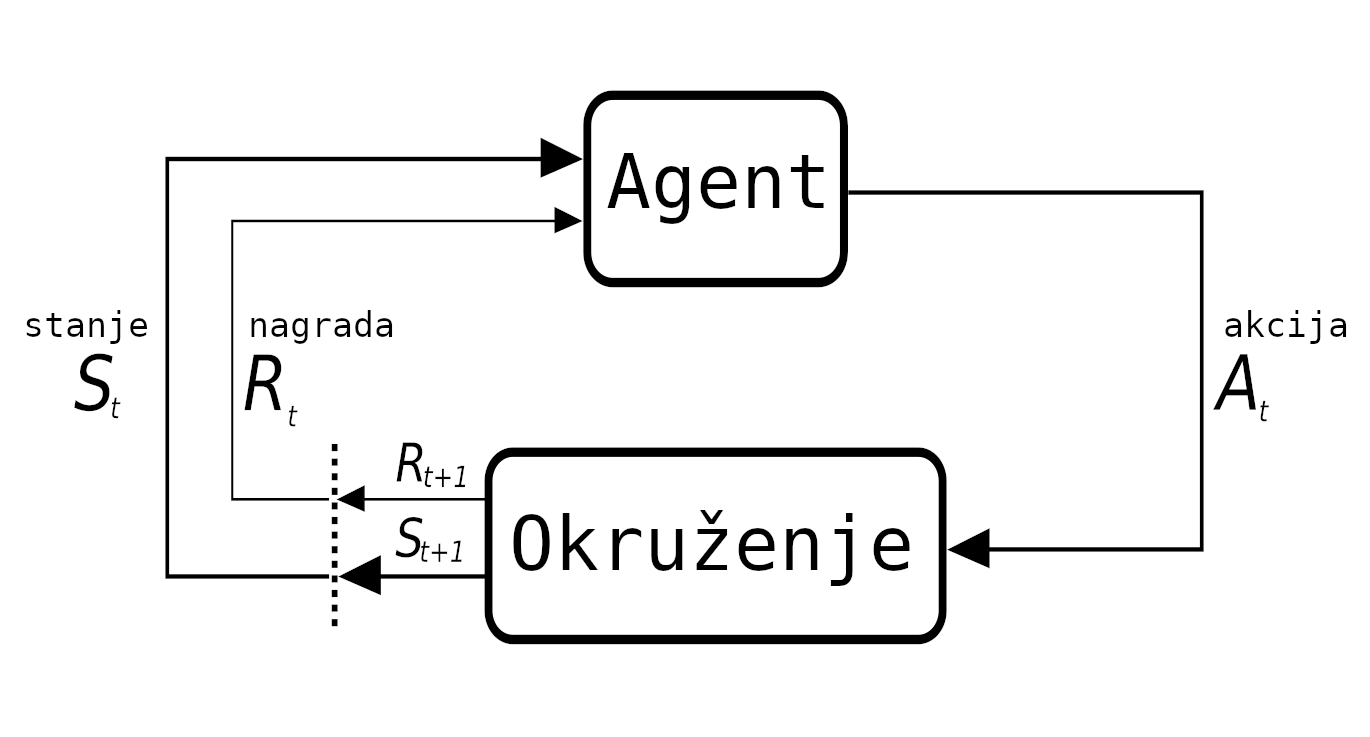
\includegraphics[width=0.8\linewidth,clip=]{images/mdp_diagram.png}%
	\figcaption{Diagram markovog procesa odlučivanja}%
	\label{fig:mdp_diagram}%
\end{minipage}
\\[\intextsep]

\subsection{Nagrada}
Očekivana nagrada $G_t$ se računa kao zbroj svih budućih nagrada $G_T = R_{t+1}+R_{t+2}+R_{t+3}+ ... + R_T$, gdje $R_T$ predstavlja nagradu u konačnom stanju okruženja. Prolaženjem jednom od početnog stanja do krajnog naziva se \emph{epizoda}, tako da pokretanjem nove epizode okruženje se ponovno namjesti na neko određeno stanje neovisno o tome kako je prijašnja epizoda završila. Međutim kako je agentu važnija neposredna nagrada, a osim toga postoje okruženja u kojima se neprekidno prelazi iz stanja u stanje i okruženje ne posjeduje konačno stanje, uvodi se pojam \emph{popust budućih nagrada}. Tako da svaku sljedeću buduću nagradu uzme sve manje u obzir. Ovakva očekivana nagrada se definira kao $R_{t+1} + \gamma R_{t+2} + \gamma ^2 R_{t+3}+...$, gdje gamma predstavlja stopu popusta budućih nagrada, $0 \leq \gamma \leq 1$, tako da je sada $G_T$ opisan jednadžbom~\ref{eq:suma_budućih_nagrada_s_popustom}.
\begin{equation}\label{eq:suma_budućih_nagrada_s_popustom}
	G_T = \sum_{k=0}^{\infty} \gamma^k R_{t+k+1}
\end{equation}

\subsection{Politike i funkcije vrijednosti}
Politika određuje agentov sljedeći potez, kroz skupljanje iskustva ta politika se može mijenjati. Označava se sa $\pi$ i definira distribuciju vjerojatnosti preko $a \in A(s)$ za svaki $s \in S$, tako da konačne vjerojatnosti svake akcije $a = A_t$ u stanju $s = S_t$ su opisane politikom $\pi(a|s)$.
Za opisivanje agentu dali se nalazi u dobrom stanju ili opisivanje agentu koliko je dobra akcija za neko stanje zadužene su funkcije vrijednosti. Koliko je dobro stanje, odnosno koliko je dobra neka akcija u nekom stanju agentu se daje do znanja pomoću vrijednosti očekivane nagrade. Funkcije vrijednosti se definiraju u odnosu na policu, pošto ona utječe na donošenje agentove odluke.
Jedna od funkcija vrijednosti je funkcija vrijednosti stanja i pomoću nje agent dobije informaciju o očekivanoj nagradi, dok prati policu $\pi$, počevši od stanja $s$ u trenutku $t$. Formalno se označava matematičkom jednadžbom~\ref{eq:state_value_function}.
\begin{equation}\label{eq:state_value_function}
	\begin{split}
		v_\pi(s) &= \mathbb{E}_\pi[G_t | S_t = s] \\
				 &= \mathbb{E}_\pi\left[\sum_{k=0}^{\infty} \gamma^k R_{t+k+1} | S_t = s\right]
     \end{split}
\end{equation}
S druge strane postoji funkcija vrijednosti akcija $q_\pi(s, a)$ koja opisuje koliko je dobra akcija $a$ u stanju $s$ dok se prati politika $\pi$. Tako da funkcija računa vrijednost očekivane nagrade za svaku akciju i definirana je matematičkom jednadžbom~\ref{eq:action_value_function}.
\begin{equation}\label{eq:action_value_function}
\begin{split}
q_\pi(s, a) &= \mathbb{E}_\pi[G_t | S_t = s, A_t = a] \\
&= \mathbb{E}_\pi\left[\sum_{k=0}^{\infty} \gamma^k R_{t+k+1} | S_t = s, A_t = a\right]
\end{split}
\end{equation}
Slovo $q$ opisuje kvalitetu (eng. \textit{quality}) određene akcije i često se vrijednost naziva q-vrijednost, te funkcija koja je daje q-funkcijom. U jednadžbama~\ref{eq:state_value_function} i ~\ref{eq:action_value_function} $\mathbb{E}_\pi$ definira očekivanu vrijednost, u ovom slučaju očekivanu nagradu, slučajne variable praćenjem politike $\pi$.

\subsubsection{Optimalne politike i funkcije vrijednosti}
Jedna od osnovnih značajki pojačanog učenja koja se ističe, je da algoritam ima neki definirani cilj, prema kojemu teži. Glavni cilj je pronalaženje optimalne politike, koju će agent pratiti, kako bi doveo nagradu do najveće moguće razine. Neka politika $\pi$ se smatra boljom od neke druge politike $\pi'$, ili bar jednako dobrom, ako za sva moguća stanja nudi višu, ili jednaku nagradu za agenta. Optimalna politika je ona koja za sva moguća stanja daje najveću nagradu i kada ne postoji neka druga politika koja za neko stanje daje veću nagradu. Također optimalna politika posjeduje njoj pripadajuću optimalnu funkciju vrijednosti stanja, odnosno optimalnu funkciju vrijednosti akcija. Optimalne funkcije se bilježe oznakom $v_*$ gdje je $v_*(s) = \max_\pi v_\pi(s)$ za funkciju vrijednosti stanja, a za funkcije vrijednosti akcija $q_*$ gdje je $q_*(s, a) = \max_\pi q_\pi(s, a)$ i to za sva $s \in S$, te u slučaju funkcije vrijednosti akcija još i za sva $a \in A$.

\subsection{Bellmanova jednadžba optimalnosti}
U nastavnom djelu ovoga rada usredočenje će biti na $q_*$, tako da se $v_*$ neće razrađivati. To ne znači da to nije primjenjivo za $v_*$, ali izrada agenta ide u smjeru q-učenja (eng. \textit{q-learning}), pa je sav daljan opis prilagođen tome. 
Po Bellmanovoj jednadžbi, koju bi trebao svaki algoritam kojemu je cilj pronalaženje optimalne funkcije vrijednosti zadovoljiti, svaka očekivana nagrada jednaka je trenutačnoj nagradi dodana na maksimalne buduće nagrade s popustom. Ima za zadatak pronaći $q_*$ koja zadovoljava jednadžbu~\ref{eq:bellman_optimality_equation}.
\begin{equation}\label{eq:bellman_optimality_equation}
q_*(s, a) = \mathbb{E}\left[R_{t+1} + \gamma\max_{a'}q_*(s', a')\right]
\end{equation}
Trenutačno stanje i akcija predstavljeni su sa $s$ i $a$, iz kojih proizlazi nagrada $R_{t+1}$. Pa je toj nagradi za bilo koje buduće stanje $s'$ i buduće akcije $a'$ dodana vrijednost maksimalne buduće nagrade s popustom. Pošto se donosi optimalnu akciju u stanju $s$, očekuje se da će se u sljedećemu stanju $s'$ moći izvršiti optimalna akciju $a'$.

\subsection{Q-Učenje}
Ideja q-učenja jest tablica u kojoj je svaki redak određeno stanje u okolini, a svaki stupac određena akcija za tu okolini. Tako da se u svakoj ćeliji nalazi q-vrijednost za određenog para stanja i akcije. Potrebno je odrediti početne q-vrijednosti, za koje nema neko čvrsto pravilo. Neki smisleni pristup je postaviti ih na nulu pošto agent još nije posjetio niti jedno stanje i nema nikakvih informacija o okolini. Neka istraživanja su pokazala da optimističnim pristupom na početno stanje, znači svakoj akciji u novom stanju se dodijeli najveća q-vrijednost, donijelo je bolje rezultate učenja. Prolaženjem kroz stanja okoline i izvršavanjem akcije se te q-vrijednosti ažuriraju, tako da češćim izvršavanjem iste akcije u nekom stanju ta q-vrijednost se sve više približava stvarnoj. Za ažuriranje q-vrijednosti u tablici koristi se Bellmannova jednadžba optimalnosti~\ref{eq:bellman_optimality_equation}. Pošto tablica u početku nema korisnih informacija o tome koje akcije poduzeti uvode se pojmovi istraživanja (eng. \textit{exploration}) i iskorištavanja (eng. \textit{exploitation}). U fazi istraživanja agent donese nasumičnu odluku, tako da u sljedećemu stanju primi nagradu i ovisno o tome može ažurirati q-vrijednost u tablici. Istraživanje služi za prikupljanje informacija o okolini kako bi se u buduće moglo donijeti što bolju odluku. U fazi iskorištavanja agent izvrši po njemu najbolju akciju, odnosno pronađe redak u q-tablici koji odgovara trenutačnom stanju i ovisno o tome koja akcija sadrži najvišu q-vrijednost, ta je akcija izabrana. Ta faza služi za prikupljanje najvišu moguću nagradu, što je ipak i agentov glavni zadatak. 

\subsubsection{Epsilon pohlepna strategija}
Potreban je neki omjer koji raspoređuje koliko i kada će se istraživati, odnosno iskorištavati. Želi se izbjeći istraživanje kada se posjeduje dovoljno informacija o okolini i izostati maksimalnoj nagradi, a također se želi izbjeći iskorištavati s nedovoljno informacija o okolini, što isto tako dovodi do neuspješnog prikupljanje maksimalne nagrade. Taj omjer u epsilon pohlepnoj strategiji (eng. \textit{epsilon greedy strategy}) je $\epsilon$ i broj je između 0 i 1. Odluka se donosi tako da se nasumično generira broj između 0 i 1, te ako je taj broj veći od $\epsilon$ onda se iskorištava, znači izabere se akcija koja bi trebala donijeti najvišu nagradu. Ako je manji onda se istražuje i izvrši se nasumična akcija, što dovodi do zaključka da sa $\epsilon = 1$ je 100\% sigurno da će se istraživati a kada je $\epsilon = 0$ se neće nikako. Kako se situacije razlikuju, da li agent posjećuje svoje prvo stanje ili je već neko vrijeme proveo u okolini i prošao dosta stanja, mora se prema tome i prilagoditi $\epsilon$. Za prilagođavanje se koristi stopa propadajućeg epsilona (eng. \textit{epsilon decay rate}), tako da na početku je $\epsilon = 1$ i vremenom opada i sve više se približava 0. Znači da je na početku agentu veći prioritet istraživati okolinu a vremenom sve više i više ju iskorištava. Po terminologiji algoritama se smatra nekim algoritmom \emph{pohlepnim} kada uzme u obzir samo neposrednu vrijednost, odnosno nagradu, u obzir bez da se razmatraju dugoročne posljedice. Pa se zbog toga kaže da agent vremenom postane pohlepan. Najčešće $\epsilon$ nikad ne dosegne vrijednost nule, nego ga se prestane smanjivati u trenutku kada $\epsilon = 0.1$, tako da u 10\% slučajeva agent i dalje istražuje, kako mu ne bi nešto promaklo.

\subsubsection{Ažuriranje q-vrijednosti}
Kada se agent uči snalaziti u okolini, kroz svako stanje koje prolazi izvrši neku akciju i ovisno o nagradi ažurira q-vrijednost u tablici. Koristi se Bellmanova jednadžba optimalnosti kako bi se q-vrijednosti u tablici približile optimalnoj $q_*$ vrijednosti. U svakom prolaženju kroz stanja se računa gubitak, odnosno razlika između $q_*(s,a)$ i $q(s, a)$, opisana jednadžbom~\ref{eq:loss_equation}. 
\begin{equation}\label{eq:loss_equation}
\begin{split}
q_*(s, a) &- q(s, a) = Gubitak \\
\mathbb{E}\left[R_{t+1} + \gamma\max_{a'}q_*(s', a')\right] &- 
\mathbb{E}\left[\sum_{k=0}^{\infty}\gamma^kR_{t+k+1}\right] = Gubitak
\end{split}
\end{equation}
S tim da se izračunata nova q-vrijednost ne pohranjuje izravno u tablicu. Agent bi trebao češće prolaziti isto stanje kako bi se mogao efektivnije približiti optimalnoj q-vrijednosti. Uvodi se novi parametar stope učenja (eng. \textit{learning rate}), koji određuje koliko će se nova vrijednost uzeti u obzir u odnosu na staru, te se označava sa  $\alpha$. Stopa učenja je broj između 0 i 1, gdje 1 znači da će nova q-vrijednost u potpunosti biti izračunata u tom trenutku a stara se neće uzeti u obzir, tj. bit će pregažena. Kako agent sve češće prolazi kroz stanja skuplja sve više iskustva i poželjno je da prijašnja iskustva uzme u obzir, tako da stvori novo iskustvo koje sadrži sažete informacije o starim iskustvima i novim. Potpuni izračun za ažuriranje nove q-vrijednosti prikazan je jednadžbom~\ref{eq:new_q_value_equation}, te iterativnim postupkom ažuriranja q-funkcija bi trebala konvergirati optimalnoj, iz čega proizlazi optimalna politika.
\begin{equation}\label{eq:new_q_value_equation}
q^{novi}(s, a) = (1 - \alpha) \cdot \underbrace{q(s, a)}_{\parbox{3em}{\footnotesize\centering staro iskustvo}} + \alpha
\overbrace{\left(R_{t+1} + \gamma\max_{a'}q(s', a')\right)}^{\parbox{3em}{\footnotesize\centering novo iskustvo}}
\end{equation}

Primjer q-učenja u Pythonu s kojim se uspješno učilo igru križić-kružić dan je u ispisu~\ref{q_learning} koji se nalazi u dodatku.

%\pythonexternal[caption={Standardno q-učenje},label=q_learning]{code/q_learning.py}

Klasa agenta naslijeđena je od bazne klase \pythoninline{Base} koja je apstraktna klasa dana u ispisu~\ref{q_learning_base_class}. Definira potpis metode \pythoninline{observe_environment}, \pythoninline{choose_action} te \pythoninline{prepare_for_episode}. 

\pythonexternal[caption=Bazna klasa agenta, label=q_learning_base_class]{code/q_learning_agent_base.py}
\iffalse
Metoda \pythoninline{prepare_for_episode} priprema agenta za novu epizodu i u ovom slučaju samo poništava vrijednosti koje su bile pohranjene u varijablama koje predstavljaju prethodno stanje i akciju. Nadalje metoda \pythoninline{observe_environment} dodaje stanje u tablicu, a ako je prvi put posjećena, poziva funkciju \pythoninline{_update_q_table} i ažurira varijable trenutnog stanja i stope istraživanja. U ovoj cijeloj klasi najzanimljivija je funkcija \pythoninline{_update_q_table} u kojoj se pomoću Bellmanove jednadžbe optimalnosti ažuriranja ćelija u tablici. Još među bitnim metodama je \pythoninline{choose_action}, koja ovisno o tome dali se istražuje ili iskorištava stanje donese odluku o sljedećoj akciji. 
\fi
Ova implementacija q-učenja očekuje okruženje \pythoninline{ObservableEnvironment} što je jako jednostavna klasa vidljiva u ispisu~\ref{q_learning_observable_environment}. Sadrži tri podatka: stanje, nagrada i to, da li je posljedno stanje u epizodi.

\pythonexternal[caption={Očekivano okruženje q-učenja},label={q_learning_observable_environment}]{code/q_learning_observable_env.py}

Može se primijetiti da nije obična klasa, pošto nema niti jedne metode, nego je zapravo struktura, a to se u Pythonu postiže nasljeđivanjem \pythoninline{NamedTuple}. Na ovaj način se generalizirao postupak q-učenja, da nije strogo vezan za križić-kružić, nego je u stanju učiti bilo koje okruženje koje prosljeđuje agentu informacije o stanju na ovakav način.

\subsection{Neuronska mreža}
U ovom području strojnog učenja se istražuju i primjenjuju umjetne neuronske mreže (eng. \textit{artificial neural networks}). Neuronske mreže na jednoj apstraktnoj razini imitiraju rad i strukturu mozga. Mozak posjeduje ogromnu mrežu stanica, nazvanih neuroni, koji su međusobno povezani. Svaki neuron preko svojih hvataljki prima signal od drugih neurona, obrađuje i prosljeđuje dalje drugim neuronima za daljnju obradu. Što je češća razmjena signala između dva neurona, to njihova veza postaje čvršća te se tako utvrđuju pojmovi. Umjetna neuronska mreža složena je u slojevima, tako da je svaki neuron povezan s neuronima iz sljedećeg sloja a nikako iz istog. Mrežu s više od dva sloja smatra se dubokom. Posebni slojevi su ulazni i izlazni slojevi, gdje ulazni slojevi primaju podatke a izlazni daju neki zaključak. Između njih se može nalaziti nekoliko skrivenih slojeva, tako da sirovi podaci stižu samo prvom sloju neurona, koji obrađeni signal usmjeravaju drugom sloju. Takav signal prolazi kroz nekoliko slojeva prije nego se mogu donijeti zaključci. Postoje različite vrste slojeva koje na drugačiji način obrađuju podatke. Osnovni sloj koji se najčešće koristi je potpuno povezani sloj (eng. \textit{fully connected layer}), ponekad i nazvan gusti sloj (eng. \textit{dense layer}). Kod računalne neuronske mreže svaki neuron je neka funkcija, koja prima neki podatak kao ulaz, obrađuje ga te izbaci na izlazu obrađeni podatak koji se šalje sljedećem neuronu na ulaz. Cijela neuronska mreža je kompozicija mnogih funkcija što je također čini funkcijom. Svakom podatku koji ulazi u neuron pridodani su parametri, često nazvani i težine (eng. \textit{weights}), pa se tijekom treninga mijenjaju parametri tako da se postigne što bolja točnost na izlazu. Na izlazu svakog neurona stoji aktivacijska funkcija koja brojem između nula i jedan opisuje koliko se taj neuron aktivira, tako da nula znači da se neuron nije aktivirao a jedan da se u potpunosti aktivirao. U ovom području jako do izražaja dolaze elementi iz linearne algebre, pošto su parametri i aktivacije vektori, matrice ili tenzori. 

\subsubsection{Učenje neuronske mreže}
Glavni cilj učenja neuronske mreže je pronalaženje optimalnih parametara koji najbolje pretvaraju ulazne podatke u željeni izlaz. Postupak se odvija tako da se za neki ulaz u mrežu usporedi izlaz sa željenim izlazom, izračuna se razlika i na osnovu toga se ažuriraju parametri u neuronskoj mreži, tako da za sljedeći put za isti ili sličan ulaz ova razlika bude što manja. Prije početka učenja parametri se inicijaliziraju s nasumičnim vrijednostima. Za izračun razlike koristi se funkcija gubitaka (eng. \textit{loss function}) koja kao ulaz prima izlaz neuronske mreže i željeni izlaz. S nasumičnim parametrima je ova razlika ogromna, a vremenom se ažuriranjem parametara teži za što manjom razlikom, odnosno da gubitak bude što bliži nuli. Gubitak koji se često koristi je funkcija srednje kvadratne pogreške (eng. \textit{mean squared error}) i opisana je formulom~\ref{eq:mean_squared_error} gdje je $y$ željeni izlaz a $\hat{y}$ izlaz koju je neuronska mreža izbacila. 
\begin{equation}\label{eq:mean_squared_error}
\frac{1}{n}\sum_{i=1}^{n}(y_i - \hat{y}_i)^2
\end{equation}
Nakon izračuna gubitka se povratnom propagacijom (eng. \textit{backpropagation}) ažuriraju svi parametri u neuronskoj mreži tako da se spuštanjem po gradijentu (eng. \textit{gradient descent}) funkcije gubitaka povećavaju ili smanjivaju vrijednosti parametara. Prema tome za koliko se u svakoj povratnoj propagaciji parametri mjenjaju, se unaprijed definira stopa učenja. Za ubrzavanje konvergencije gubitka koriste se optimizacije kao stohastično spuštanje po gradijentu (eng. \textit{stochastic gradient descent}) koji nasumičnim uzorkivanjem računa gubitak samo na maloj skupini podataka s kojom dobije neku procjenu stvarne funkcije gubitaka. Dodatno pomoću momentuma, koji oponaša akceleracijsku silu na stopi učenja, znači što češće se vrijednosti mijenjaju u nekom smjeru to su koraci veći, se taj postupak još ubrzaje. Vremenom su se mnogo raznih optimizacija razvile i ne postoji neko pravilo pomoću kojega se može odrediti što se koristi u kojemu trenutku, nego se izvode pokusi s raznim metodama i promatraju rezultati pomoću kojih se onda izabere metoda za daljnji rad. Od svih metoda koje se koriste u dubokom učenju, funkcija srednje kvadratne vrijednosti i stohastično spuštanje po gradijentu su na neki način početna točka s kojom se uči.

\subsubsection{Duboka Q-mreža}
S obzirom na to da neko okruženje posjeduje ogromnu količinu stanja, te pohranjivanje svih stanja bi moglo vrlo lako prelaziti raspoloživu memoriju računala, s dubokom se umjetnom neuronskom mrežom aproksimira q-tablicu. Sastavljena je tako, da na ulaznom sloju ulazi stanje a na izlaznom sloju se svakoj akciji pridodijeli njezinu q-vrijednost. S dubokom q-mrežom se također računa optimalna q-vrijednost pomoću Bellmannove jednadžbe optimalnosti.
